\documentclass[11p]{article}
% Packages
\usepackage{amsmath}
\usepackage{graphicx}
\usepackage[swedish]{babel}
\usepackage[utf8]{inputenc}
\usepackage[T1]{fontenc}

\usepackage[
    backend=biber,
    style=authoryear-ibid,
    sorting=ynt
]{biblatex}
%Källor
\addbibresource{mall.bib}
\graphicspath{ {./images/} }

\title{PMmall \\ \small Fysik 1}
\author{Endo Axelsson }
\date{\today}


\begin{document}

    \begin{titlepage}
        \begin{center}
            \vspace*{1cm}

            \Huge
            \textbf{Title}

            \vspace{0.5cm}
            \LARGE
            Subtitle

            \vspace{1.5cm}

            \textbf{Author Name}

            \vfill

            Ett PM om energiförsörjning \\
            Fysik 1

            \vspace{0.8cm}

            
\includegraphics[width=0.4\textwidth]{../images/NTI Gymnasiet_Symbol_print_svart.png}

            \Large
            Teknikprogrammet\\
            NTI Gymnasiet\\
            Umeå\\
            \today

        \end{center}
    \end{titlepage}
% Om arbetet är långt har det en innehållsförteckning, annars kan den utelämnas
    \tableofcontents
    \newpage

    \section{Inledning}
    Vi behöver en ny och mer miljövänlig energikälla för jordens hälsa långsiktigt.
    En energikälla som inte är  beroende av olja och brännbara fossiler.
    Detta är ett relevant ämne som diskuterass runtom hela världen för att minska växthuseffekten.
    Vilken källa är bäst och hur mycket av det finns det?
    Dem naturliga energikällorna är temat som pratas mycket om och vindkraft är en av dem.
    Men som allt annat så har allt positivt också något negativt och vindkraft är inte ett undantag.
    Så det finns det såklart frågor runtom vindkraften också.
    \subsection{frågeställningar}
    \begin{enumerate}
        \item Vindkraft, så fungerar det
        \item Globala och lokala miljöpåverkan av vindkraft
        \item Vindkraftens påverkan på områden och ekonomi
        \item Vindkraft, land eller vatten?
    \end{enumerate}

    \section{Resultat}

    \subsection{Vindkraft, så fungerar det}

  Vindkraftens funktion är i princip rätt så simpelt, Som namnet utger så kommer energin från vinden.
  Vinden blåser mot vindkraftverken och möter rotorbladen, detta tillför mekanisk energi som får
  bladet att rotera sig.
  Bladet sitter samman med en maskinhus som i sin del genererar elelektrisk
  energi.
  Denna energin åker ner till en transformator där energin justeras så att den kan tillföras
  vidare till hus och andra grejer.

  Det praktiska är att vindriktningen faktist inte spelar någon  roll.
   Alla vindkraftverk som inte är i äldre versioner har turbiner som roterar sig till rätt riktning.
    \begin{figure}
        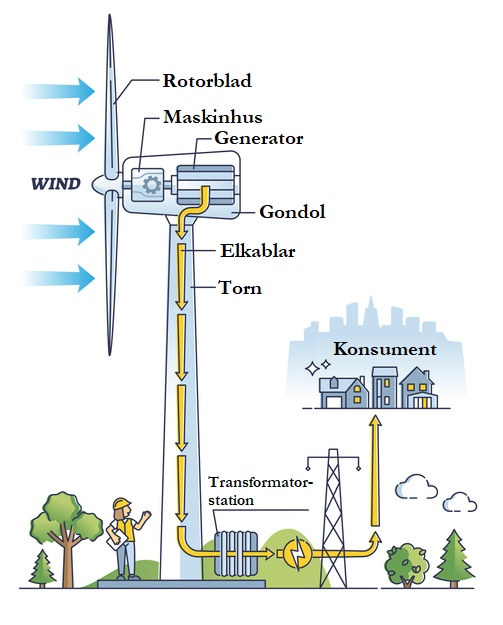
\includegraphics[width=0.6\textwidth]{../images/vindhur.jpg}
        \caption{funktionen simplifierad. Källa: Ugglasno.se}
    \end{figure}
    \subsection{Globala och lokala miljöpåverkan av vindkraft}
    Miljöpåverkan på olika saker är en stor fråga som är aktuellt.
    Fokuset är att hitta en energikälla som inte är begränsad av och påverkar miljön lika mycket som dem som är vanligast.
    När man snackar om energikällor så tänker man ofta på mängden energin som tillverkas och produktionen.
    Där inte mycket enrgi som andra,
    Själva monteringen och konstrueringen är det som kostar som mest och påverka miljön.
    när allt väl är uppe så är vindkraftverk väldigt bra, långsiktigt så är det en stabil källa om man endast tänker på miljö perspektivet.
    Som \parencite{ugglansfysik} tar upp på deras sida ,för det första så är det lite underhåll, ingen restfall efter, inte lika stor påverkan på naturlivet runt om, energin är förnybar, gratis och den största fördelen är att den inte bidrar till växthuseffekten ()


    \subsection{Vindkraftens påverkan på samhället och ekonomi}
   I en artikel så nämner \textcite{divaportal} om
    natur folk tycker att det är fult
    Stör djurliv?
    Kostar mycket för att bygga upp för mängden energin man får tillbaka (det finns billigare alternativ kortsiktigt)
    dock så kräver det lite underhåll som sagt så det kräver mindre pengar under en längre period
   Beroende av andra källor när det är vindstilla
    \subsection{Vindkraft, land eller vatten?}

    \includegraphics[width=1\textwidth]{../images/vindterräng.jpg}

    \subsection{}

    \section{Slutsatser}
    Här kan du dra slutsatser eller sammanfatta ditt resultat

    JAG FORM ÅSIKTER.

% Mer saker som du kan ha nytta av.

    \section{Referenser}
    Referenser i text kan skrivas på två sätt: Enligt \textcite{Jens} kan man använde två typer av referenser, inbäddade i texten eller efter ett fakta \parencite{Fraenkel}. Ett till test för att se hur det ser ut \parencite[sid 55]{fermi}.

    \section{Annat som kan vara bra att veta}
    Om du vill ha kodstil och få med alla tecken kan du använda verbatim. då kan du skriva \verb|abcd!"#| utan problem...





\end{document}
